\documentclass{beamer}
\usetheme{Singapore}
\usepackage{tikz}
\usepackage{color}
\usetikzlibrary{positioning}
\usetikzlibrary{chains}
\usetikzlibrary{calc}
\usetikzlibrary{backgrounds}
%\usepackage{amsmath}
\title[Alba] % (optional, only for long titles)
{The Alba Storage System}
\subtitle{The \textcolor{red}{AL}ternative \textcolor{red}{BA}ckend}
\author[Slootmaekers, Doms] % (optional, for multiple authors)
{J.~Doms \and R.~Slootmaekers}
\institute[Open vStorage] % (optional)
{
%  \inst{1}%
%  Institute of Computer Science\\
%  University Here
%  \and
%  \inst{2}%
%  Institute of Theoretical Philosophy\\
%  University There
}
\date[Nov 2014] % (optional)
{Internal Presentation, 2014}
\subject{Alba}

\begin{document}
\frame{\titlepage}

\begin{frame}
  \frametitle{Mark III architecture}
  \framesubtitle{ Proxy + Arakoon Namespace Manager + ASDs }
  \begin{columns}[T]
    \begin{column}[T]{5cm}
      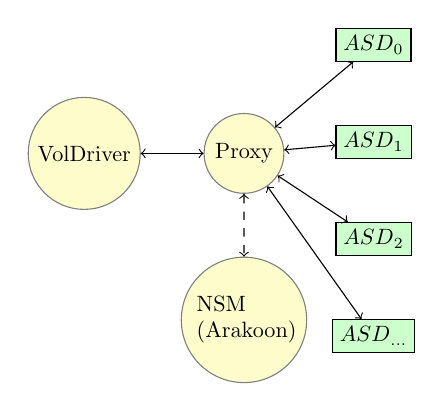
\begin{tikzpicture}[scale = 0.8, transform shape]
        \tikzset{
          my_data/.style={rectangle, fill=green!20, draw},
          my_process/.style={circle, draw = black!50, fill= yellow!20},
        }

        \node (proxy)  [my_process] {Proxy};
        \node (vd)     [my_process, left = of proxy] {VolDriver};
        \node (nsm)    [my_process, below = of proxy,
                        text width=1.5cm] {NSM (Arakoon)};
        \node (data0)  [my_data, above right = of proxy]  {$\text{ASD}_0$};
        \node (data1)  [my_data, below = of data0]        {$\text{ASD}_1$};
        \node (data2)  [my_data, below = of data1]        {$\text{ASD}_2$};
        \node (dataX)  [my_data, below = of data2]        {$\text{ASD}_{\ldots}$};

        \path[draw, <->]
        (vd) edge node [left] {} (proxy)
        ;
        \path[draw, <->]
        (proxy) edge node [left] {} (data0)
                edge node [left] {} (data1)
                edge node [left] {} (data2)
                edge node [left] {} (dataX)
        ;
        \path[draw, <->, dashed]
        (proxy) to (nsm)
        ;
      \end{tikzpicture}

    \end{column}
  \end{columns}
\end{frame}

\begin{frame}
  \frametitle{Mark III architecture}
  \framesubtitle{ Proxy + Arakoon Namespace Manager + ASDs }
  \begin{columns}[T]
    \begin{column}[T]{5cm}
      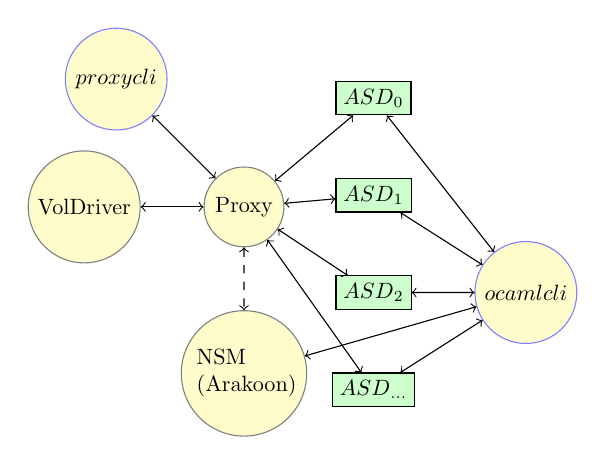
\begin{tikzpicture}[scale = 0.8, transform shape]
        \tikzset{
          my_data/.style={rectangle, fill=green!20, draw},
          my_process/.style={circle, draw = black!50, fill= yellow!20},
          my_cli/.style={circle, draw = blue!50, fill = yellow!20},
        }

        \node (proxy)  [my_process] {Proxy};
        \node (vd)     [my_process, left = of proxy] {VolDriver};
        \node (nsm)    [my_process, below = of proxy,
                        text width=1.5cm] {NSM (Arakoon)};
        \node (pcli)   [my_cli, above left = of proxy] {$\text{proxy cli}$};
        \node (data0)  [my_data, above right = of proxy]  {$\text{ASD}_0$};
        \node (data1)  [my_data, below = of data0]        {$\text{ASD}_1$};
        \node (data2)  [my_data, below = of data1]        {$\text{ASD}_2$};
        \node (dataX)  [my_data, below = of data2]        {$\text{ASD}_{\ldots}$};
        \node (ocli)   [my_cli, right = of data2] {$\text{ocaml cli}$};

        \path[draw, <->]
        (vd) edge node [left] {} (proxy)
        ;
        \path[draw, <->]
        (proxy) edge node [left] {} (data0)
                edge node [left] {} (data1)
                edge node [left] {} (data2)
                edge node [left] {} (dataX)
        ;
        \path[draw, <->, dashed]
        (proxy) to (nsm)
        ;

        \path[draw, <->]
        (pcli) edge node [left] {} (proxy)
        ;

        \path[draw, <->]
        (ocli) edge node [left] {} (nsm)
               edge node [left] {} (data0)
               edge node [left] {} (data1)
               edge node [left] {} (data2)
               edge node [left] {} (dataX)
        ;
      \end{tikzpicture}

    \end{column}
     \begin{column}{5cm} % alternative top-align that's better for graphics
       \begin{block}{OCaml cli also useful for implementing}
       \begin{itemize}[<+(1)->]
         \item Repair
         \item Gc
         \item Fragments cleanup (from deleted/overwritten objects)
       \end{itemize}
       \end{block}
     \end{column}

  \end{columns}
\end{frame}

\begin{frame}
  \frametitle{Current status}
  \framesubtitle{ What works }
  \begin{columns}[T]
    \begin{column}[T]{10cm}

      \begin{itemize}
      \item upload/download/delete/list object
        from both the proxy client and ocaml client
      \item most of the 'backend\_test' and some of the 'volumedriver\_test' tests
      \item can remove an asd and downloads keep on working
      \end{itemize}


    \end{column}
  \end{columns}
\end{frame}

\begin{frame}
  \frametitle{Current Status}
  \framesubtitle{ What still needs to be done }
  \begin{itemize}
    \item need a manager for the namespace managers
      (currently only 1 namespace is supported)
    \item non happy paths (e.g. error on network connections, slow asds, ...)
    \item keep the deployment unit in mind for fragment placement
    \item gc, repair process, obsolete fragment cleanup (some initial work has been done)
    \item detect dead disks, decommission them
    \item deployment
    \item possible performance optimisations
    \item others: mostly complete list available as todo.txt in alba repo
  \end{itemize}
\end{frame}

\end{document}
